\documentclass{standalone}

\usepackage{tikz}
\usepackage{amsmath}
\usepackage{pgfplots}
\usetikzlibrary{arrows}

\begin{document}
	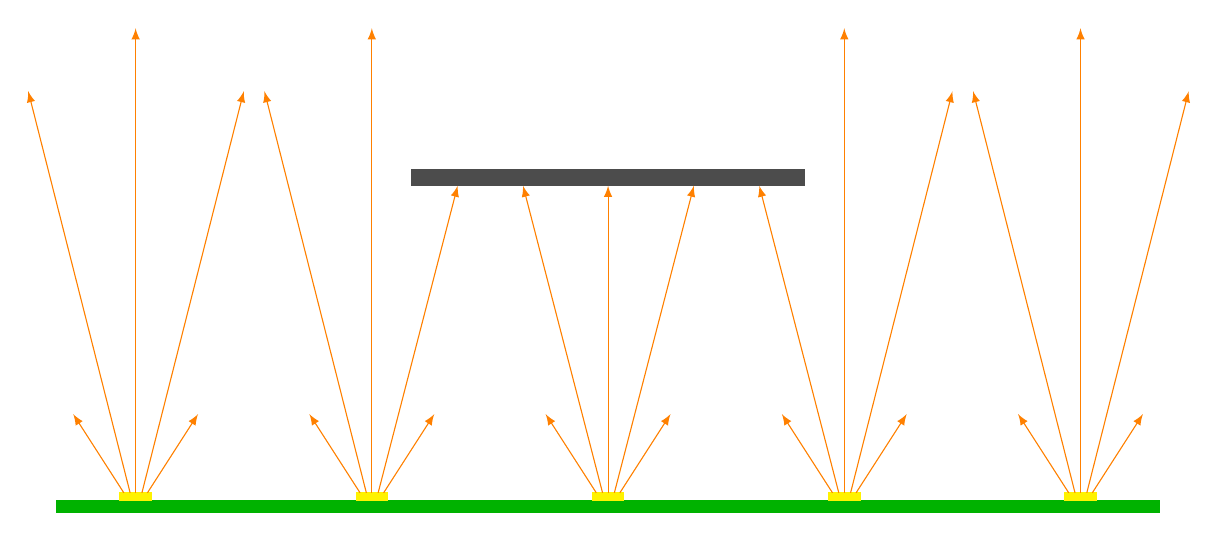
\begin{tikzpicture}[>=latex]
		% print
		\filldraw[green!70!black] (0,0) rectangle (14,-0.15);
		
		% LEDs
		\filldraw[yellow] (0.8,0) rectangle (1.2,0.1);
		\filldraw[yellow] (3.8,0) rectangle (4.2,0.1);
		\filldraw[yellow] (6.8,0) rectangle (7.2,0.1);
		\filldraw[yellow] (9.8,0) rectangle (10.2,0.1);
		\filldraw[yellow] (12.8,0) rectangle (13.2,0.1);
		
		% Object
		\filldraw[black!70!white] (4.5,4) rectangle (9.5,4.2);
		
		% Lichstrahlen (12 und 35 grad)
		%mitte
		\draw[->, orange] (7, 0.1)--(7, 4);
		\draw[->, orange] (6.93, 0.1)--++(-1.01, 3.9);
		\draw[->, orange] (6.85,0.1)--++(-0.643,1);
		\draw[->, orange] (7.08, 0.1)--++(1.01, 3.9);
		\draw[->, orange] (7.15,0.1)--++(0.643,1);
		
		%mitte rechts
		\draw[->, orange] (10, 0.1)--(10, 6);
		\draw[->, orange] (9.93, 0.1)--++(-1.01, 3.9);
		\draw[->, orange] (9.85,0.1)--++(-0.643,1);
		\draw[->, orange] (10.08, 0.1)--++(1.294, 5.1);
		\draw[->, orange] (10.15,0.1)--++(0.643,1);
		
		%mitte links
		\draw[->, orange] (4, 0.1)--(4, 6);
		\draw[->, orange] (3.93, 0.1)--++(-1.294, 5.1);
		\draw[->, orange] (3.85,0.1)--++(-0.643,1);
		\draw[->, orange] (4.08, 0.1)--++(1.01, 3.9);
		\draw[->, orange] (4.15,0.1)--++(0.643,1);
		
		% links
		\draw[->, orange] (1, 0.1)--(1, 6);
		\draw[->, orange] (0.93, 0.1)--++(-1.294, 5.1);
		\draw[->, orange] (0.85,0.1)--++(-0.643,1);
		\draw[->, orange] (1.08, 0.1)--++(1.294, 5.1);
		\draw[->, orange] (1.15,0.1)--++(0.643,1);
		
		% rechts
		\draw[->, orange] (13, 0.1)--(13, 6);
		\draw[->, orange] (12.93, 0.1)--++(-1.294, 5.1);
		\draw[->, orange] (12.85,0.1)--++(-0.643,1);
		\draw[->, orange] (13.08, 0.1)--++(1.294, 5.1);
		\draw[->, orange] (13.15,0.1)--++(0.643,1);
		
	\end{tikzpicture}
\end{document}